\documentclass[11pt,AutoFakeBold]{article}
\usepackage{xeCJK}  % 调用 xeCJK 宏包
\usepackage{fullpage}  
\usepackage{graphicx}
\usepackage{amssymb}
\usepackage{fancyvrb}
\usepackage{CJK} 
\usepackage{listings} 
\usepackage{xcolor}
\usepackage{amsmath}
\usepackage{titlesec}
\usepackage{enumerate}
\usepackage{enumitem}
\usepackage{booktabs}
\usepackage[colorlinks=true,linkcolor=cyan]{hyperref}
\usepackage{geometry}
\geometry{a4paper,left=2cm,right=2cm,top=2cm,bottom=2cm}
\setlist[enumerate,1]{label=(\arabic*),itemsep=15pt}
\renewcommand{\baselinestretch}{1.5}
\usepackage{fontspec}
\setmainfont{Times New Roman}
\lstset{keywordstyle=\color{blue}, %%设置关键字颜色  
        commentstyle=\color[cmyk]{1,0,1,0}, %% 设置注释颜色  
        frame=single, %% 设置边框格式  
        escapeinside=``, %% 逃逸字符(1左面的键),用于显示中文  
        extendedchars=false, %% 解决代码跨页时,章节标题,页眉等汉字不显示的问题  
        xleftmargin=2em,xrightmargin=2em, aboveskip=1em,, %% 设置边距   
        showspaces=false %% 不显示空格  
        tabsize=4, %% 设置tab空格数 
       }       
\setCJKmainfont{NSimSun}% 设置 CJK 主字体为 SimSun (宋体)
\usepackage{tikz}


\title{运筹学第二次作业\\第四章\quad 整数规划}
\author{\normalsize 蒋文馨 \quad 16342067}
\date{\today}

\begin{document}
\maketitle
\renewcommand{\contentsname}{目录}
\tableofcontents


\section{工厂制造数学模型}
\textbf{解:}设工厂制造A,B,C三种容器的数量分别为$x_1,x_2,x_3$只, 记
总利润为$f$, 则所研究问题可写成
$$\begin{array}{l}
\max f=4 x_{1}+5 x_{2}+6 x_3 \\
\left\{\begin{array}{l}
2x_{1}+4x_{2}+8x_3 \leqslant 500 \\
2x_{1}+3x_{2}+4x_3 \leqslant 300 \\
x_{1}+2x_{2}+3x_3\leqslant 1000 \\
x_{i} \geqslant 0,\text {且为整数}, i=1,2,3
\end{array}\right.
\end{array}$$


\section{篮球联赛出场阵容数学模型}
\textbf{解:}首先, 记$c_i,i=1,2,\cdots,8$为号码为i的队员的身高. 
平均身高为$f$.\\
引进变量$x_i,i=1,2,\cdots,8$, 规定
$$x_i=\left\{\begin{array}{l}
        1,\quad \text{当号码为i的队员上场时}\\
        0,\quad \text{当号码为i的队员不上场时}
\end{array}\right.$$
问题的数学形式可以写成:
$$\begin{array}{l}
\max f=\frac{\sum_{i=1}^8 c_ix_i}{\sum_{i=1}^8 x_i} \\
\left\{\begin{array}{l}
x_{1}+x_{2}= 1 \\
x_{6}+x_{7}+x_8\geqslant 1 \\
x_{1}+x_4+x_6 \leqslant 0 \\
x_{2}+x_6 = 1 \\
x_{i} = 0\text{ 或 }1,\quad i=1,2,\dots,8
\end{array}\right.
\end{array}$$


\section{分支定界法}
        $$\begin{array}{l}
        \min f=-5 x_{1}+x_{2}-2 x_{3}+5 \\
        \left\{\begin{array}{l}
        -2 x_{1}+x_{2}-x_{3}+x_{4}=7/2  \qquad(*)\\
        2 x_{1}+x_{2}+x_{3} +x_{5}=2 \qquad (**)\\
        x_{j} \geqslant 0, \quad j=1,2, \cdots, 5 \\
        x_{3}, x_{4} \text { 为整数 }
        \end{array}\right.\end{array}$$ 
\textbf{解:}由(**)知$x_3$可取值为0,1,2.
\begin{enumerate}
        \item 当$x_3=2$时, 由(**)知$x_1=x_2=x_5=0$, 故
        由(*)知$x_4=9/2$不是整数, 不符合题意.
        \item 当$x_3=1$时, 原问题可以化为
        $$\begin{array}{l}
        \min f=-5 x_{1}+x_{2}+3 \\
        \left\{\begin{array}{l}
        -2 x_{1}+x_{2}+x_{4}=9/2\\
        2 x_{1}+x_{2}+x_{5}=1\\
        x_{j} \geqslant 0, \quad j=1,2, 4, 5 \\
        x_{4} \text { 为整数 }
        \end{array}\right.\end{array}$$
        进一步, 
        $$\begin{array}{l}
        \min f=-3 x_{1}-x_{4}+15/2 \\
        \left\{\begin{array}{l}
        -2 x_{1}+x_{2}+x_{4}=9/2\\
        -4 x_{1}+x_{4}-x_5=7/2\\
        2 x_{1}+x_{2}+x_{5}=1\\
        x_{j} \geqslant 0, \quad j=1,2, 4, 5 \\
        x_{4} \text { 为整数 }
        \end{array}\right.\end{array}$$
        由此,
        $$\begin{array}{l}
        \min f=-3 x_{1}-x_{4}+15/2 \\
        \left\{\begin{array}{l}
        -2 x_{1}+x_{4} \leqslant 9/2\\
        -4 x_{1}+x_{4}\geqslant 7/2\\
        0\leqslant x_{1}\leqslant 1\\
        x_{4} \text { 为正整数 }
        \end{array}\right.\end{array}$$

        对于上述问题的松弛问题, 利用图解法求出可行域, 如图\ref{1}所示.
        其中, 紫色区域为松弛问题可行域, 点A为满足约束条件的最优解. 此时
        $\mathbf{x}=(3/8,1/4 ,1,5,0), f_{min}=11/8.$ 

\begin{figure}[!htbp]
        \begin{center}
        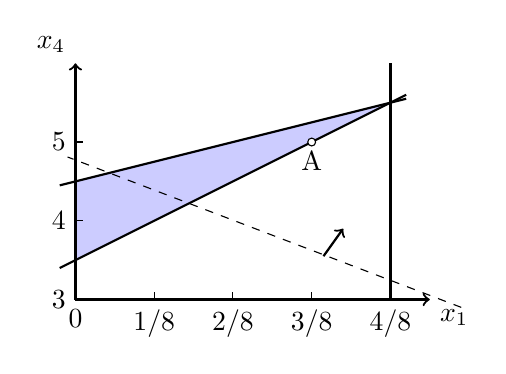
\begin{tikzpicture}{c}
        %画x和y轴坐标
        \fill[blue!20!white] (0,0.5)--(0,1.5)--(4,2.5);
        \draw[thick,->] (0,0) -- (4.5,0) node[anchor=north west] {$x_1$};
        \draw[thick,->] (0,0) -- (0,3) node[anchor=south east] {$x_4$};
        \draw[thick] (4,0) -- (4,3);
        \draw[thick] (4.2,2.55) -- (-0.2,1.45);
        \draw[thick] (-0.2,0.4) -- (4.2,2.6);
        \draw[thick,->] (3.15,0.55) -- (3.4,0.9);
        \draw[dashed] (4.9,-0.1) -- (-0.1,1.81);
        %画刻度3
        \foreach \x in {0,1,2}
        {
                \draw[xshift=\x cm] (0,0) -- (0,0.1);
                \draw[yshift=\x cm] (0,0) -- (0.1,0);
        };  
        \draw[xshift=3 cm] (0,0) -- (0,0.1);
        %标坐标原点
        \node[below] at (0,0){0};
        \node[below] at (3,2){A};
        \draw[color=black, fill=white] (3,2) circle (.05);
        %标x轴刻度值
        \foreach \x in {1,2,...,4}
                \node[below] at(\x,0){\x/8};
        % 标注y轴刻度
        \node[left] at(0,0){3};
        \node[left] at(0,1){4};
        \node[left] at(0,2){5};
        \end{tikzpicture}
        \caption{$x_3=1$时可行域示意图}
        \label{1}                 
\end{center}
\end{figure}

\item 当$x_3=0$时, 同理可得
        $$\begin{array}{l}
        \min f=-3 x_{1}-x_{4}+17/2 \\
        \left\{\begin{array}{l}
        -2 x_{1}+x_{4} \leqslant 7/2\\
        -4 x_{1}+x_{4}\geqslant 3/2\\
        0\leqslant x_{1}\leqslant 1\\
        x_{4} \text { 为正整数 }
        \end{array}\right.\end{array}$$

        对于上述问题的松弛问题, 利用图解法求出可行域, 如图\ref{2}所示.
        其中, 紫色区域为松弛问题可行域, 点A为满足约束条件的最优解. 此时
        $\mathbf{x}=(7/8,1/4,0,5,0), f_{min}=7/8$.

\begin{figure}[!htbp]
        \begin{center}
        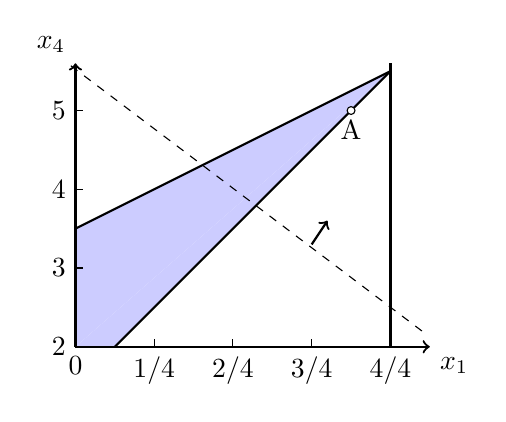
\begin{tikzpicture}{c}
        \fill[blue!20!white] (0,0)--(0,1.5)--(4,3.5);
        \fill[blue!20!white] (0,0)--(0.5,0)--(4,3.5);
        %画x和y轴坐标
        \draw[thick,->] (0,0) -- (4.5,0) node[anchor=north west] {$x_1$};
        \draw[thick,->] (0,0) -- (0,3.6) node[anchor=south east] {$x_4$};
        \draw[thick] (4,0) -- (4,3.6);
        \draw[thick] (0.5,0) -- (4,3.5);
        \draw[thick] (0,1.5) -- (4,3.5);
        \draw[thick,->] (3,1.3) -- (3.2,1.6);
        \draw[dashed] (4.4,0.2) -- (-0.1,3.6);
        %画刻度
        \foreach \x in {0,1,2,3}
        {
                \draw[xshift=\x cm] (0,0) -- (0,0.1);
                \draw[yshift=\x cm] (0,0) -- (0.1,0);
        };  
        %标坐标原点
        \node[below] at (0,0){0};
        \node[below] at (7/2,3){A};
        \draw[color=black, fill=white] (7/2,3) circle (.05);
        %标x轴刻度值
        \foreach \x in {1,2,...,4}
                \node[below] at(\x,0){\x/4};
        % 标注y轴刻度
        \node[left] at(0,0){2};
        \node[left] at(0,1){3};
        \node[left] at(0,2){4};
        \node[left] at(0,3){5};
        
        \end{tikzpicture}
        \caption{$x_3=0$时可行域示意图}
        \label{2}                 
\end{center}
\end{figure}
\end{enumerate}
 综上, 最优解为$\mathbf{x}=(7/8,1/4,0,5,0)$, 最优值为$f_{min}=7/8$.
        

\section{割平面法}
\begin{enumerate}
\item $$\begin{array}{l}
        \max f=2 x_{1}+x_{2} \\
        \left\{\begin{array}{l}
        x_{1}+x_{2} \leqslant 6 \\
        x_{1}-4 x_{2} \leqslant 2 \\
        x_{1} \geqslant 0, x_{2} \geqslant 0, \text {且全为整数 }
        \end{array}\right.
        \end{array} $$
 \textbf{解:}
首先, 引入松弛变量, 化为标准形式:
        $$\begin{array}{l}
        \min f'=-2 x_{1}-x_{2} \\
        \left\{\begin{array}{l}
        x_{1}+x_{2} +x_3= 6 \\
        x_{1}-4 x_{2} +x_4= 2 \\
        x_{1} \geqslant 0, x_{2} \geqslant 0, \text {且全为整数 }\\
        x_{3} \geqslant 0, x_{4} \geqslant 0
        \end{array}\right.
        \end{array} $$
利用单纯形法求得最优基为$\mathbf{B}=(\mathbf{P_1},\mathbf{P_2})$ ,
对应的单纯形表为表\ref{t1}.\\
        \begin{table}[!htbp]
        \centering
        \caption{第四题(1)单纯形表1}
        \label{t1}
        \setlength{\tabcolsep}{7mm}{
        \begin{tabular}{c|c|cccc} 
        \toprule
        \hline
             &   & $x_1$ & $x_2$ & $x_3$ & $x_4$  \\ 
        \hline
        $f'$    & -56/5 & 0   & 0    & -9/5    & -1/5       \\ 
        \hline
        $x_2$ & 4/5 & 0    & 1& 1/5 & -1/5     \\ 
        $x_1$ & 26/5 &1    & 0& 4/5 & 1/5     \\ 
        \hline
        \bottomrule
        \end{tabular}}
        \end{table}

则割平面为:\\
以$f$为源行: $\frac{1}{5}x_3+\frac{4}{5}x_4\geqslant \frac{4}{5}$\\
以$x_1$为源行: $\frac{1}{5}x_3+\frac{4}{5}x_4\geqslant \frac{4}{5}$ \\
以$x_2$为源行: $\frac{4}{5}x_3+\frac{1}{5}x_4\geqslant \frac{1}{5}$\\
前两个割平面完全相同, 割平面等价于:
$$\left\{\begin{array}{l}
         x_1\leqslant 5 \\ x_1-3x_2\leqslant 2               
\end{array}\right.$$

引入松弛变量$s_1,s_2\geqslant 0$, 得到单纯形表\ref{t2}.
        \begin{table}[!htbp]
        \centering
        \caption{第四题(1)单纯形表2}
        \label{t2}
        \setlength{\tabcolsep}{7mm}{
        \begin{tabular}{c|c|cccccc} 
        \toprule
        \hline
             &   & $x_1$ & $x_2$ & $x_3$ & $x_4$ &$s_1$&$s_2$ \\ 
        \hline
        $f'$    & -56/5 & 0   & 0    & -9/5    & -1/5  &0  &0  \\ 
        \hline
        $x_2$ & 4/5 & 0    & 1& 1/5 & -1/5 &0 &0   \\ 
        $x_1$ & 26/5 &1    & 0& 4/5 & 1/5  &0  &0 \\ 
        $s_1$ & 5& 1&0 &0&0&1&0\\
        $s_2$&2&1&-3&0&0&0&1\\
        \hline
        \bottomrule
        \end{tabular}}
        \end{table}
进一步可得单纯形表\ref{t3}.\\至此,得$x_1=5,x_2=1,f'_{min}=-11.$
故原问题最优解$x_1=5,x_2=1,f_{max}=11.$
        % \begin{table}[!htbp]
        % \centering
        % \caption{第四题(1)单纯形表3}
        % \label{t3}
        % \setlength{\tabcolsep}{7mm}{
        % \begin{tabular}{c|c|cccccc} 
        % \toprule
        % \hline
        %      &   & $x_1$ & $x_2$ & $x_3$ & $x_4$ &$s_1$&$s_2$ \\ 
        % \hline
        % $f$    & -56/5 & 0   & 0    & -9/5    & -1/5  &0  &0  \\ 
        % \hline
        % $x_2$ & 4/5 & 0    & 1& 1/5 & -1/5 &0 &0   \\ 
        % $x_1$ & 26/5 &1    & 0& 4/5 & 1/5  &0  &0 \\ 
        % $s_1$ & -1/5& 0&0 &-4/5       &-1/5      &1      &0\\
        % $s_2$ &-4/5    &0  &0     &-1/5      &-4/5      &0      &1\\
        % \hline
        % \bottomrule
        % \end{tabular}}
        % \end{table}
        \begin{table}[!htbp]
        \centering
        \caption{第四题(1)单纯形表3}
        \label{t3}
        \setlength{\tabcolsep}{7mm}{
        \begin{tabular}{c|c|cccccc} 
        \toprule
        \hline
                &   & $x_1$ & $x_2$ & $x_3$ & $x_4$ &$s_1$&$s_2$ \\ 
        \hline
        $f$    & -11 & 0   & 0    & -7/4    & 0  &0  &-1/4  \\ 
        \hline
        $x_2$ & 1 & 0    & 1& 1/4 & 0 &0 &-1/4   \\ 
        $x_1$ & 5 &1    & 0& 3/4 & 0  &0  &1/4 \\ 
        $s_1$ & 0& 0&0 &3/4      &0     &1      &-1/4\\
        $s_2$ &1    &0  &0     &1/4      &1      &0      &-5/4\\
        \hline
        \bottomrule
        \end{tabular}}
        \end{table}

\item $$\begin{array}{l}
        \max f=4 x_{1}+5 x_{2} \\
        \left\{\begin{array}{l}
        3 x_{1}+2 x_{2} \leqslant 10 \\
        x_{1}+4 x_{2} \leqslant 11 \\
        x_{1} \geqslant 0, x_{2} \geqslant 0, \text {且全为整数 }
        \end{array}\right.
        \end{array}$$
 \textbf{解:}
 首先, 引入松弛变量, 化为标准形式:
 $$\begin{array}{l}
\min f'=-4 x_{1}-5 x_{2} \\
\left\{\begin{array}{l}
3 x_{1}+2 x_{2} +x_3= 10 \\
x_{1}+4 x_{2} +x_4= 11 \\
x_{1} \geqslant 0, x_{2} \geqslant 0, \text {且全为整数 }\\
x_{3} \geqslant 0, x_{4} \geqslant 0
\end{array}\right.
\end{array}$$

利用单纯形法求得最优基为$\mathbf{B}=(\mathbf{P_1},\mathbf{P_2})$ ,
对应的单纯形表为表\ref{t1}.
 \begin{table}[!htbp]
 \centering
 \caption{第四题(2)单纯形表1}
 \label{t4}
 \setlength{\tabcolsep}{7mm}{
 \begin{tabular}{c|c|cccc} 
 \toprule
 \hline
      &   & $x_1$ & $x_2$ & $x_3$ & $x_4$  \\ 
 \hline
 $f'$    & -187/10 & 0   & 0    & -11/10   & -7/10\\ 
 \hline
 $x_1$ & 9/5 & 1    & 0& 2/5 & -1/5     \\ 
 $x_2$ & 23/10 &0    & 1& -1/10 & 3/10     \\ 
 \hline
 \bottomrule
 \end{tabular}}
 \end{table}
则割平面为:\\
以$f$为源行: $3x_3+x_4\geqslant 1$\\
以$x_1$为源行: $x_3+2x_4\geqslant 2$ \\
以$x_2$为源行: $3x_3+x_4\geqslant 1$.\\
第3个式子和第1个等价, 割平面等价于:
$$\left\{\begin{array}{l}
        x_1+x_2\leqslant 4 \\ x_1+2x_2\leqslant 6               
\end{array}\right.$$

引入松弛变量$s_1,s_2\geqslant 0$, 得到单纯形表\ref{t5}.
 \begin{table}[!htbp]
 \centering
 \caption{第四题(2)单纯形表2}
 \label{t5}
 \setlength{\tabcolsep}{7mm}{
 \begin{tabular}{c|c|cccccc} 
 \toprule
 \hline
      &   & $x_1$ & $x_2$ & $x_3$ & $x_4$ &$s_1$&$s_2$ \\ 
 \hline
 $f'$    & -187/10 & 0   & 0    & -11/10   & -7/10&0&0\\ 
 \hline
 $x_1$ & 9/5 & 1    & 0& 2/5 & -1/5 &0&0  \\ 
 $x_2$ & 23/10 &0    & 1& -1/10 & 3/10 &0&0\\ 
 $s_1$ & 4& 1&1 &0&0&1&0\\
 $s_2$&6&1&2&0&0&0&1\\
 \hline
 \bottomrule
 \end{tabular}}
 \end{table}
%######################
% \begin{table}[!htbp]
% \centering
% \caption{第四题(2)单纯形表2}
% \setlength{\tabcolsep}{6.5mm}{
% \begin{tabular}{c|c|cccccc} 
% \toprule
% \hline
%         &   & $x_1$ & $x_2$ & $x_3$ & $x_4$ &$s_1$&$s_2$ \\ 
%  \hline
%  $f'$    & -187/10 & 0   & 0    & -11/10   & -7/10&0&0\\ 
%  \hline
%  $x_1$ & 9/5 & 1    & 0& 2/5 & -1/5 &0&0  \\ 
%  $x_2$ & 23/10 &0    & 1& -1/10 & 3/10 &0&0\\ 
%  $s_1$ & -1/10& 0&0 &-3/10&-1/10&1&0\\
%  $s_2$&-2/5&0&0&-1/5&-2/5&0&1\\
% \hline
% \bottomrule
% \end{tabular}}
% \end{table}

\begin{table}[!htbp]
\centering
\caption{第四题(2)单纯形表3}
\label{t6}
\setlength{\tabcolsep}{7mm}{
\begin{tabular}{c|c|cccccc} 
\toprule
\hline
&   & $x_1$ & $x_2$ & $x_3$ & $x_4$ &$s_1$&$s_2$ \\ 
\hline
$f'$    & -18 & 0   & 0    & -3/4   & 0&0&-7/4\\ 
\hline
$x_1$ & 2 & 1    & 0& 1/2 & 0 &0&-1/2  \\ 
$x_2$ & 2 &0    & 1& -1/4 & 0 &0&3/4\\ 
$s_1$ & 0& 0&0 &-1/4&0&1&-1/4\\
$x_4$&1&0&0&1/2&1&0&-5/2\\
\hline
\bottomrule
\end{tabular}}
\end{table}

进一步可得单纯形表\ref{t6}.至此,得$x_1=2,x_2=2,x_3=0,x_4=1,f'_{min}=-18$.
故原问题最优解$x_1=2,x_2=2,f_{max}=18.$

\end{enumerate}
\end{document}